\iffalse
\bibliography{../bib/thesis.bib}
\fi

\chapter{基于文件社交网络的恶意软件检测方法研究}

\section{相关研究}

\section{系统架构}
基于文件社交网络的恶意软件检测系统架构包含四个主要模块,如图\ref{fig_SysArchitecture}所示。文件列表采集模块(\textit{File List Collector})从用户的终端设备(包括个人电脑,手机和平板等智能设备)采集文件样本,同时提取出文件样本间的关联关系,并转存文件列表以及每个文件的关联关系至文件关系数据库(\textit{File Relation Database})中。文件关联图构造模块(\textit{File Relation Graph Constructor})根据关系数据库构造能够表示文件之间关联关系的文件关联图,在系统框架中起重要的作用。在文件关联图的基础之上,图特征提取和采样模块(\textit{Graph-based Feature Extractor})分析基于图的特征属性,在这些特征属性的基础之上选择一些具有重要的代表性的节点(对应的文件样本)进行人工标记,从图属性的层面提高分类器的准确率水平,使得模型更加健壮。作为系统结构的核心,基于主动学习(Active Learning)的标签传播分类器(\textit{Label Propagation Classifier})根据文件关联图学习未标记样本的标签信息(即恶意或者良性),在学习的过程中主动学习(Active Learning)选择重要的文件样本进行人工标记从而在算法层面上提高标签传播分类器的性能。

\begin{figure}[!ht]
\centering
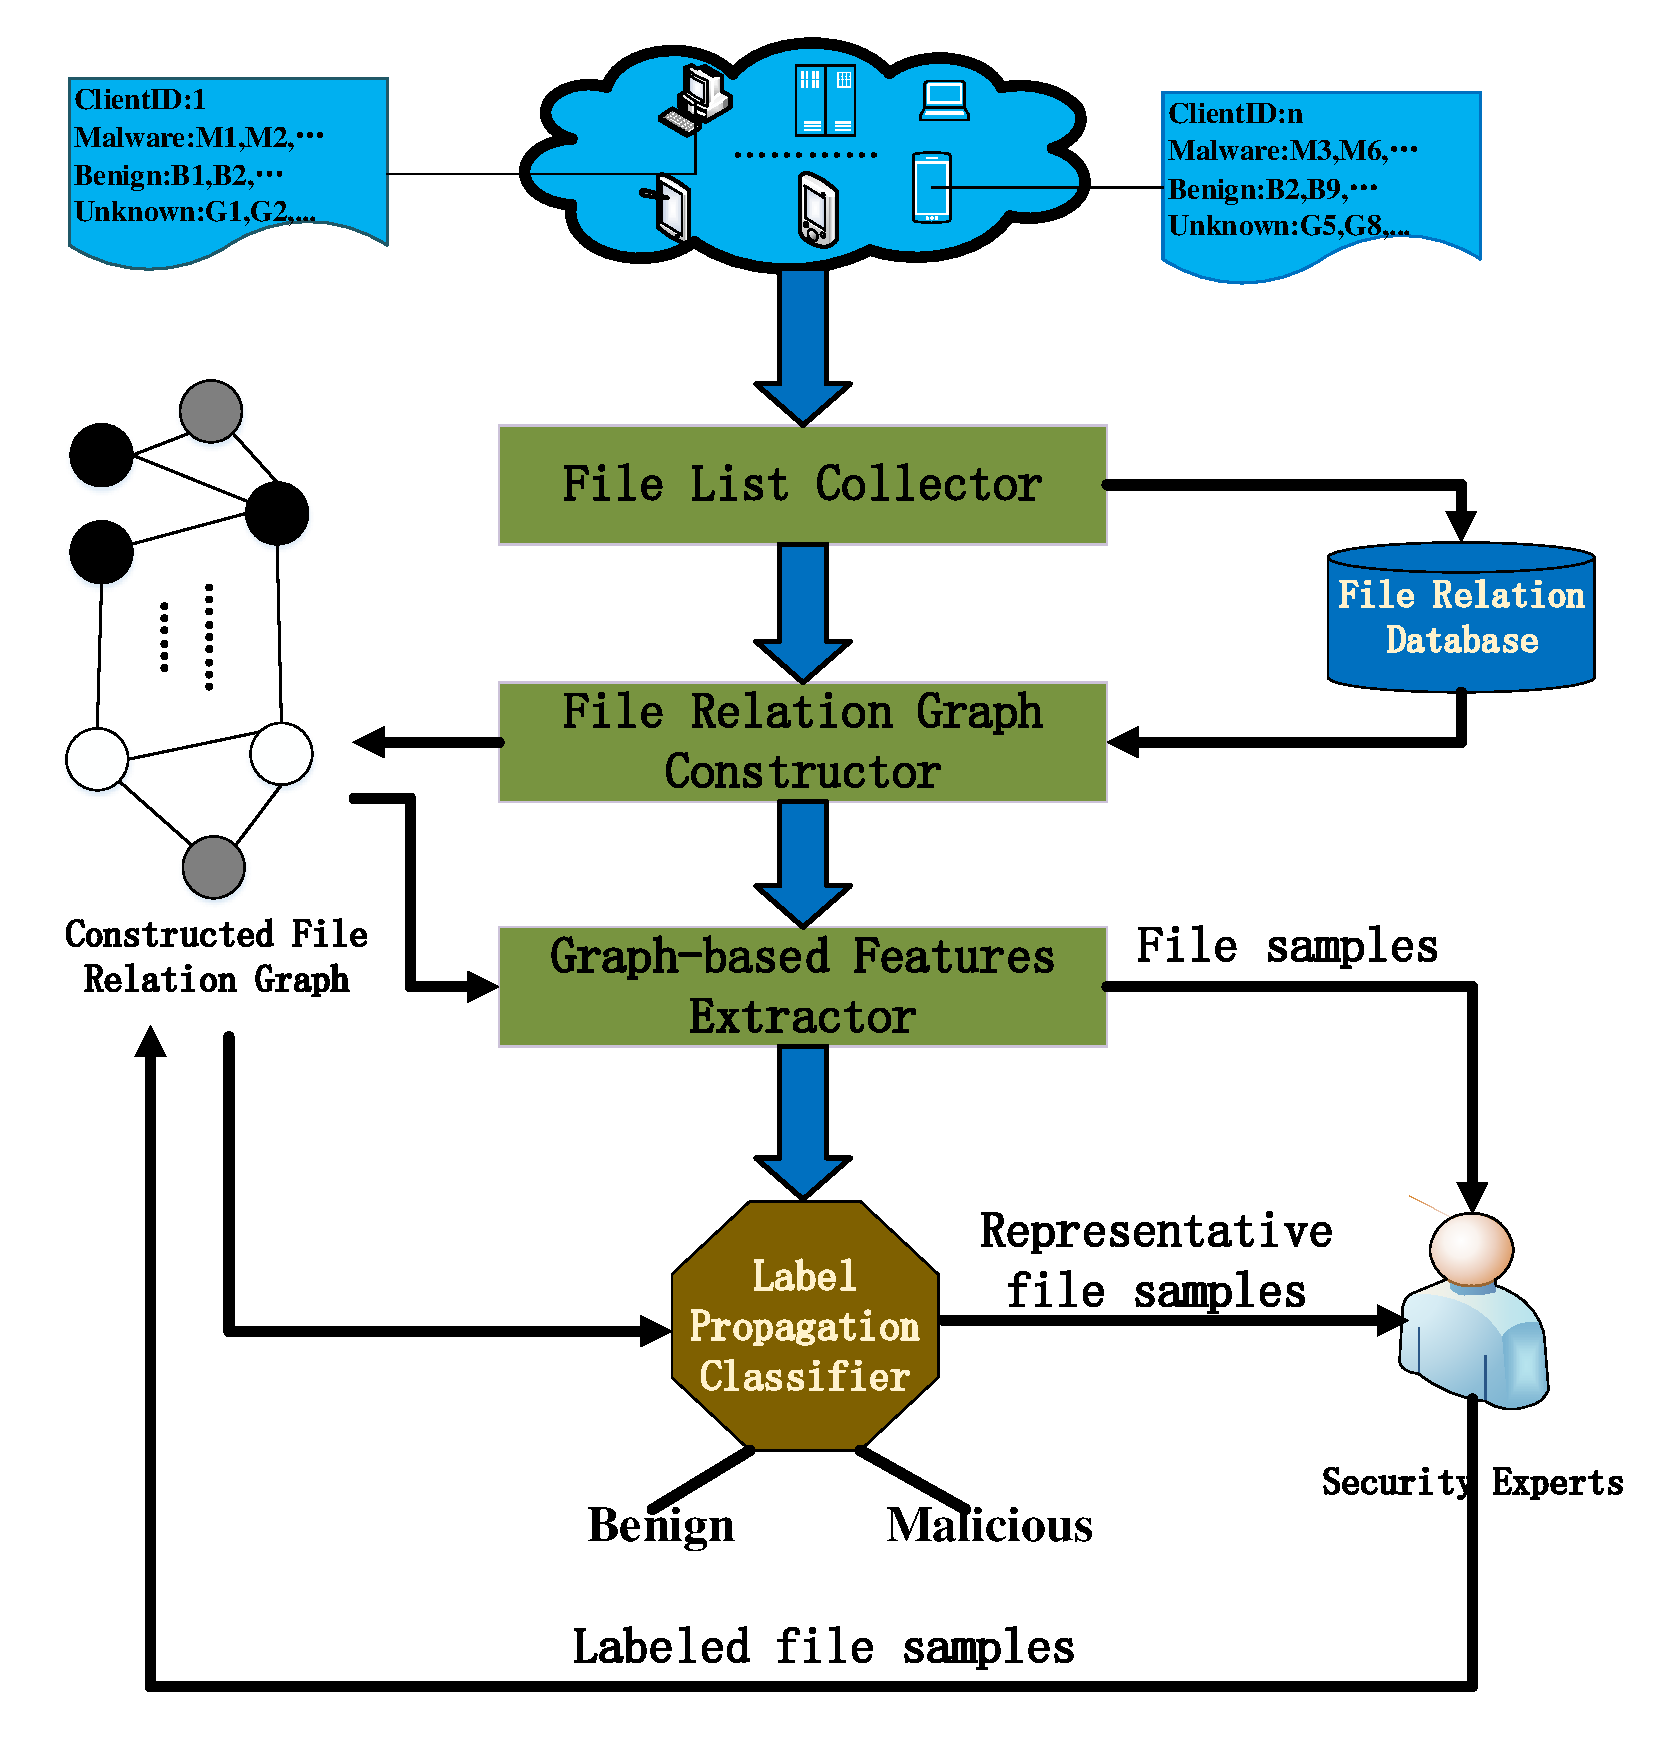
\includegraphics[width=3.5in]{img/chap3/SystemArchitecture.pdf}
\caption{总体框架}
\label{fig_SysArchitecture}
\end{figure}
\section{文件样本社交网络分析}
\subsection{文件关联图}
本章采用上一章中文件关联图的构建算法($k$近邻图)构建文件关联图,图\ref{fig:vis:1}为构建的文件关联图,图\ref{fig:vis:2}和图\ref{fig:vis:3}分别展示了其中一个恶意文件样本和良性文件样本及其它们一跳范围内的关联信息。其中,红色点为恶意软件,绿色点为良性文件,黄色点为未标记样本。
\begin{figure}[!ht]
\centering
\subfigure[文件关联图]{\label{fig:vis:1} 
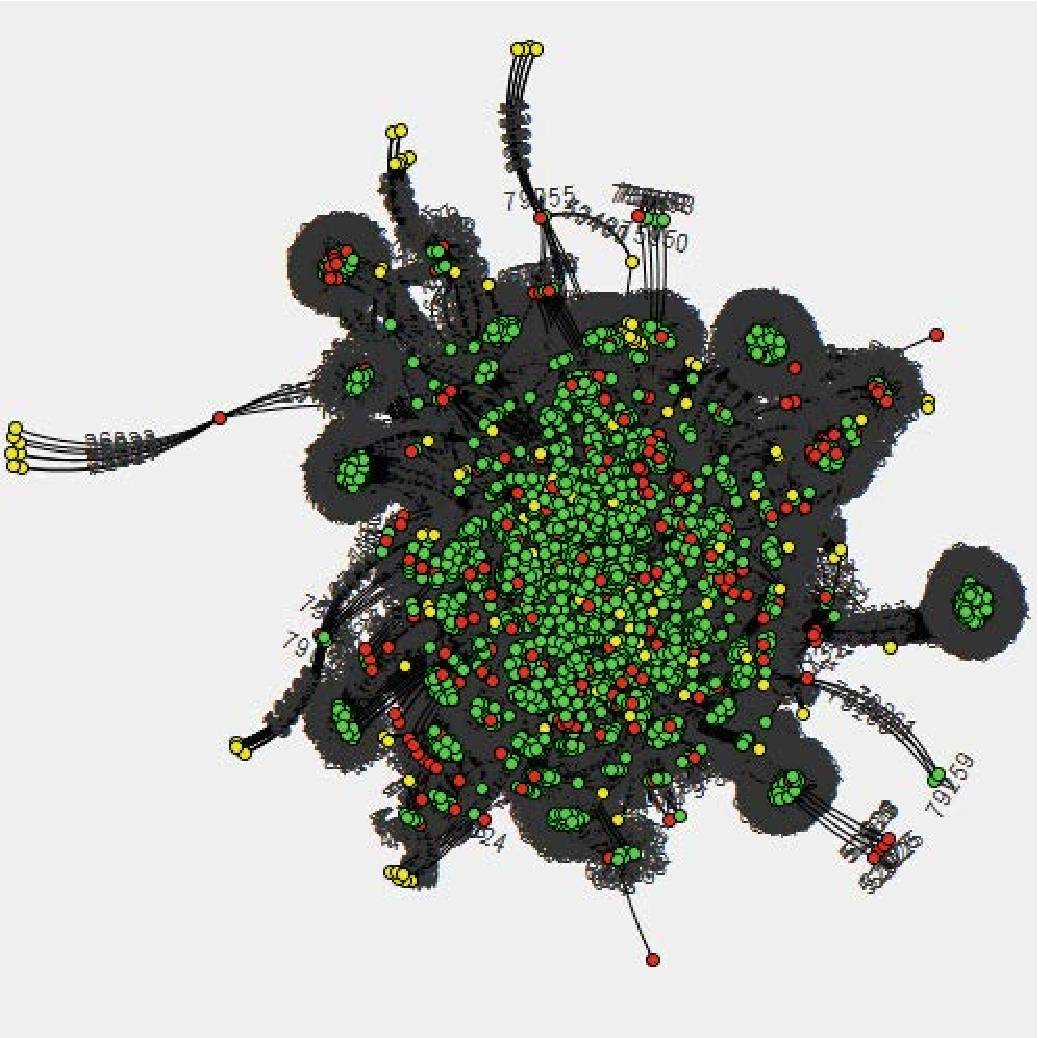
\includegraphics[width=.32\linewidth]{img/chap3/vis1.pdf}}
% \hspace{0.1in}
% \quad
\subfigure[恶意软件关联]{\label{fig:vis:2} 
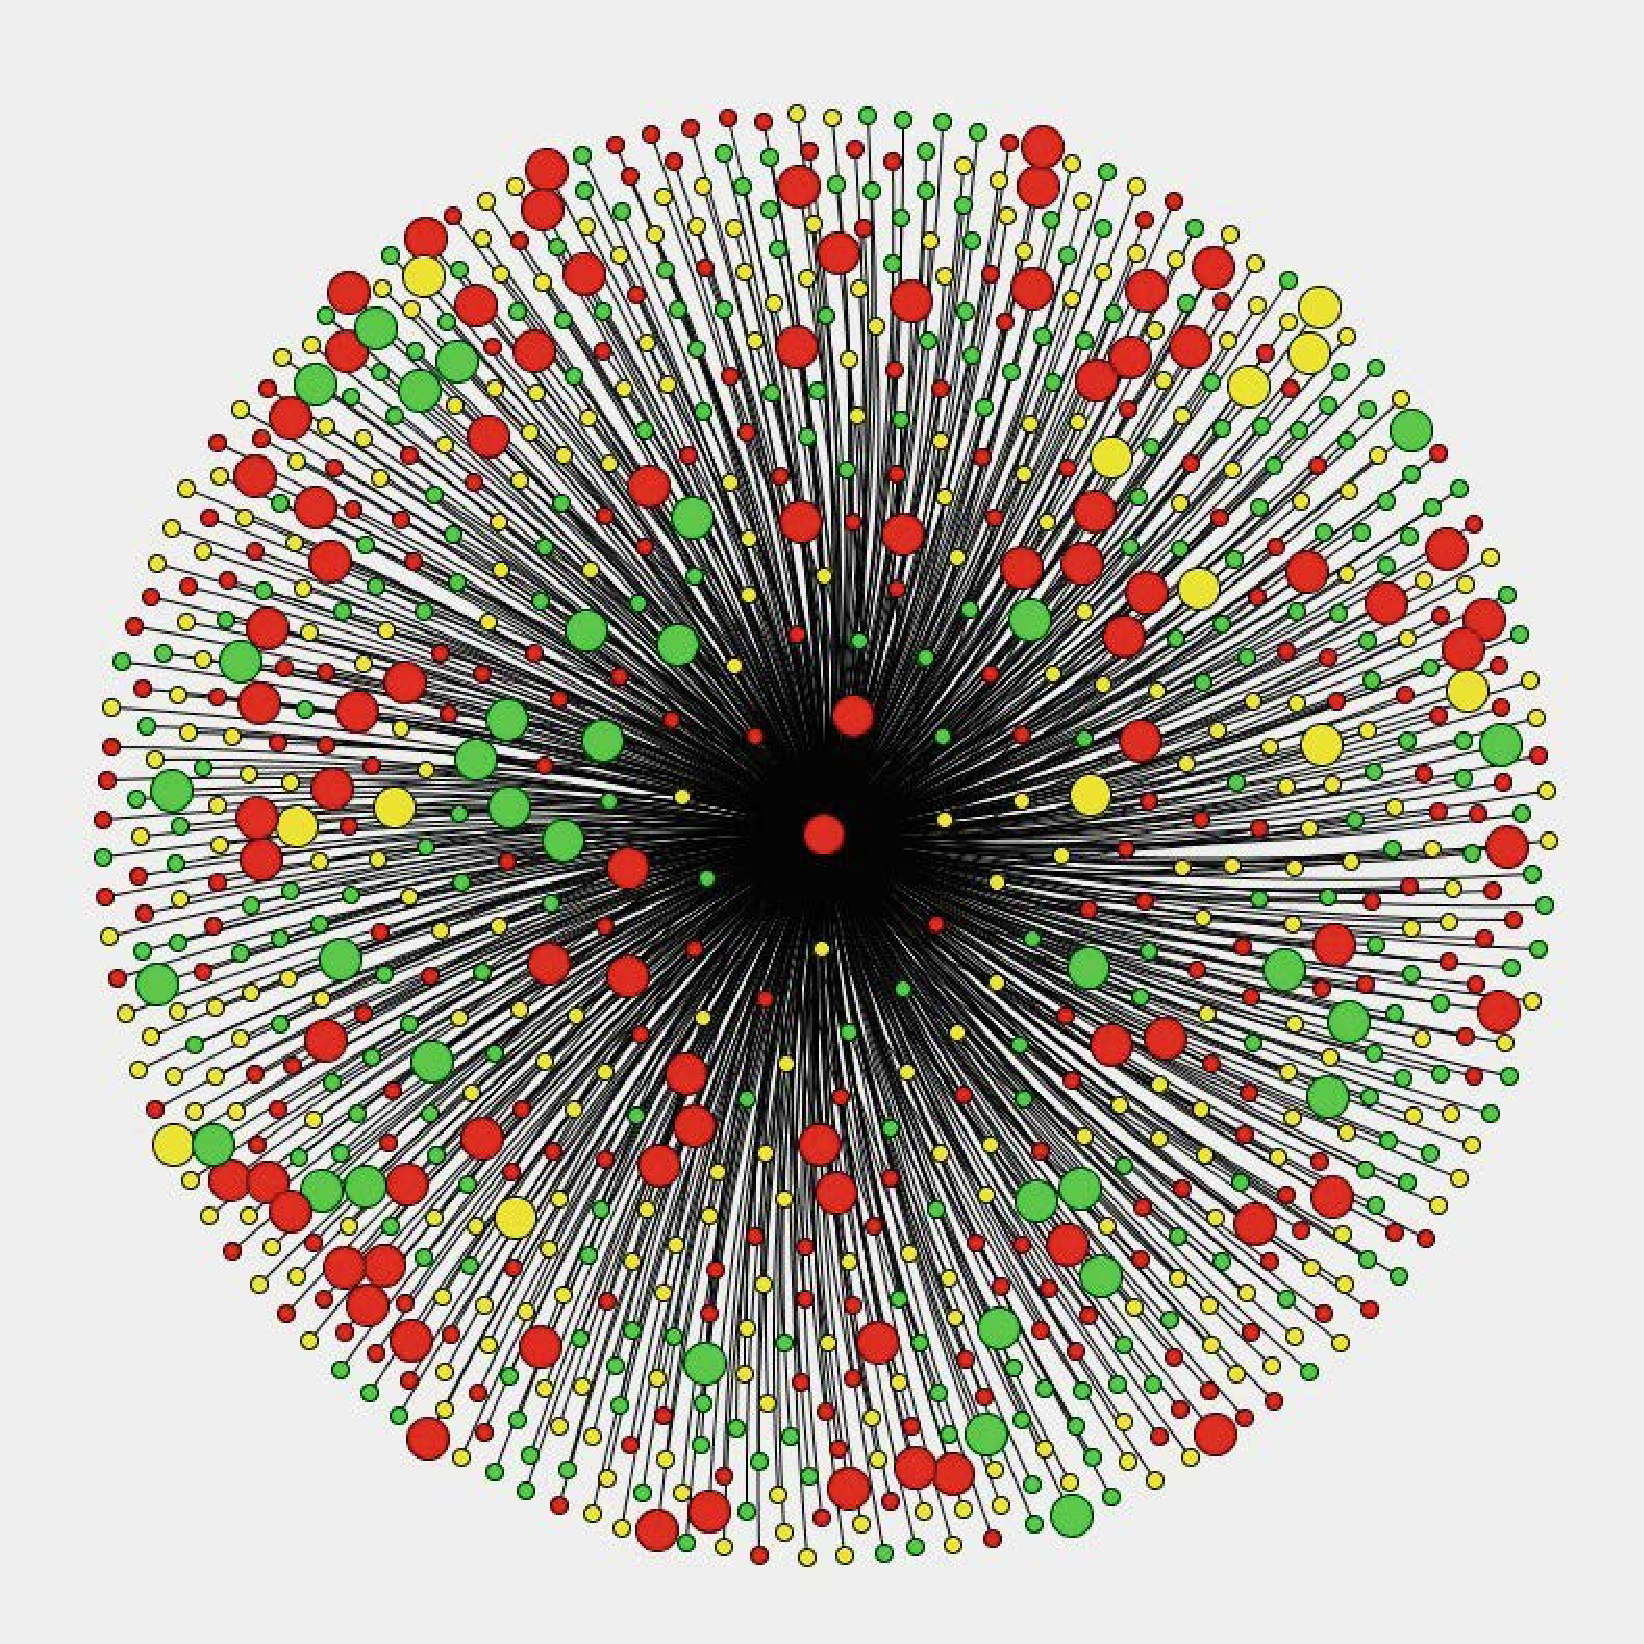
\includegraphics[width=.32\linewidth]{img/chap3/vis2.pdf}}
% \quad
\subfigure[良性文件关联]{\label{fig:vis:3} 
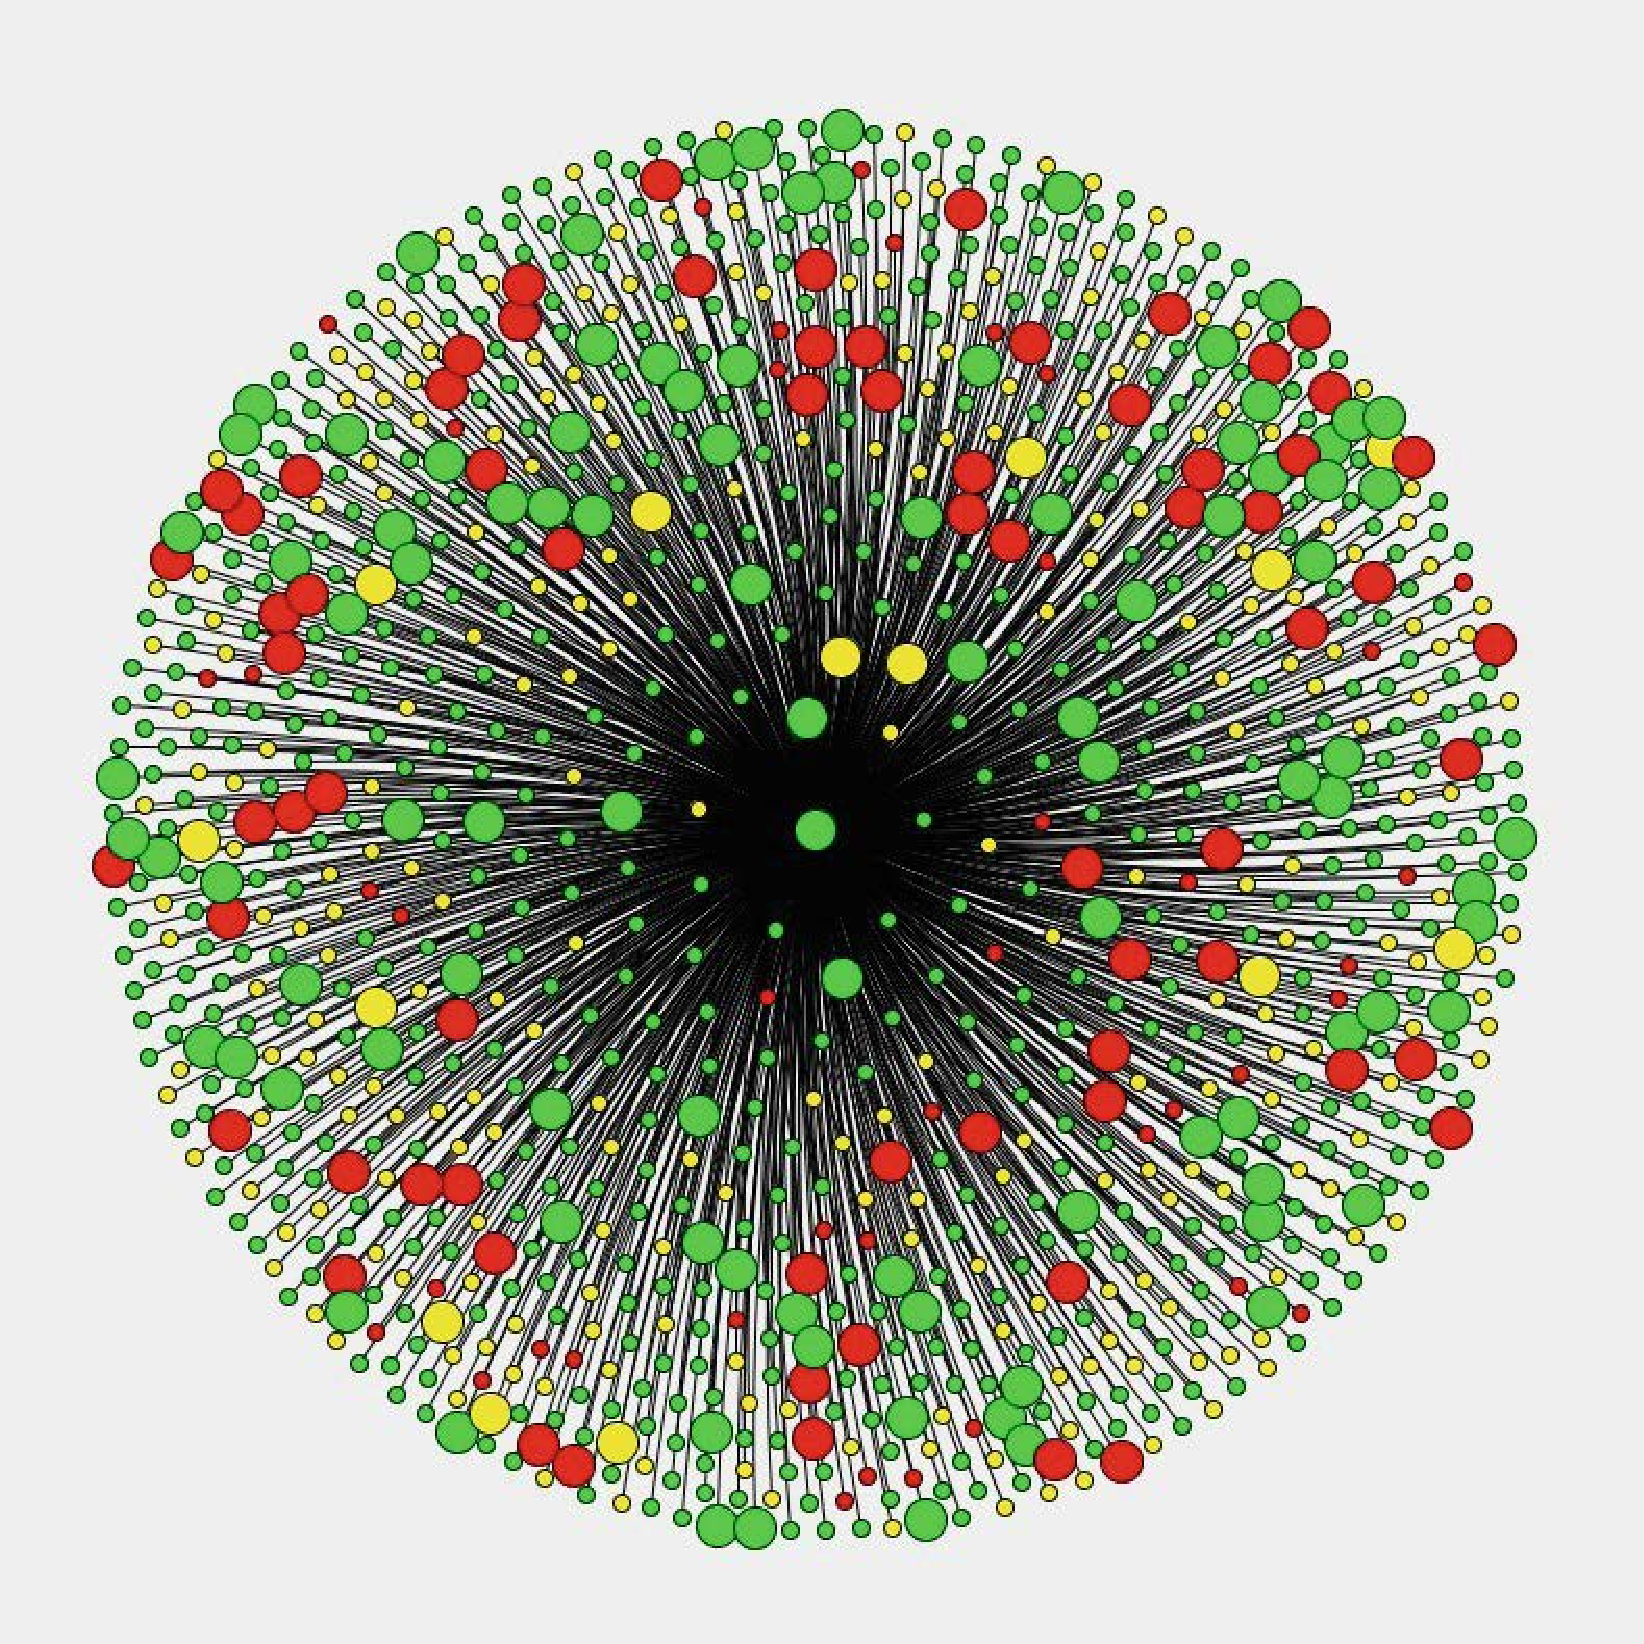
\includegraphics[width=.32\linewidth]{img/chap3/vis3.pdf}}
\caption{文件关联图可视化}
\label{fig:vis}
\end{figure}
\subsection{文件关联网络的特征属性}
\subsubsection{节点度}
在图论中,节点度是指与节点相关联的边的数量,又称为关联度。节点度能够明确的表示节点与其邻居的关联性\cite{diestel2010graph}。在文件关联图中,提出节点的恶意软件度($DoM$)和节点的良性文件度($DoB$)来分别衡量文件与不同类型文件的关联关系,根据公式分别计算:
\begin{equation}
\label{eq:domAnddob}
DoM(v)=\left | \delta_{m}^{v}  \right |, DoB(v)=\left | \delta_{b}^{v}  \right |
\end{equation}
其中,$\left | \delta_{m}^{v}  \right |$是节点$v$恶意邻居节点的数量,$\left | \delta_{b}^{v}  \right |$是节点$v$良性邻居节点的数量。古人云:近朱者赤,近墨者黑。同样的道理,在计算机网络中恶意软件的$DoM$将比$DoB$大,反之亦然。

\subsubsection{局部聚类系数}
聚类系数表示一个图形中节点聚集程度的系数,用于描述网络中节点和其邻居节点之间互相连接的紧密程度,即网络的集团化程度。聚类系数主要分为全局聚类系数、局部聚类系数和平均聚类系数。局部聚类系数表示一个节点的相邻节点形成一个团(完全图)的紧密程度,故本章采用局部聚类系数来计算文件关联图中节点的聚集能力,计算方法为\cite{watts1998collective}:
\begin{equation}
\label{eq:lccUW}
LCC(v)=\frac{2\left | e^{v} \right |}{d_{v}(d_{v}-1)},
\end{equation}
其中$\left | e^{v} \right |$为节点$v$的所有邻居节点之间的边的总数,$d_{v}$为节点$v$的度。这里的局部聚类系数$LCC$在计算时考虑了节点度以及邻居节点之间的边,能够较好的表达无权图中节点的局部紧密程度。而在带权图中,每条边上的权重衡量了每对节点之间的相似度,而在公式\ref{eq:lccUW}的计算中每个邻居节点都被平等对待,没有考虑每对节点之间的相似程度,即两点之间边的权重,因此在带权图中,计算节点的局部聚类系数时需要根据连接至节点的边的权重来计算。Jukka-Pekka Onnela等人\cite{onnela2005intensity}提出了一种基于子图强度的带权图局部聚类系数计算方法,定义为子图中边权重的几何均值:
\begin{equation}
LCC(v)=\frac{1}{d_{v}(d_{v}-1)}\sum_{i,j \in N(v)}(\hat{w}_{vi}\hat{w}_{vj}\hat{w}_{ij})^{1/3},
\end{equation}
其中,$N(v)$是节点$v$的邻居节点集合,$\hat{w}_{vi}$是经过公式\ref{eq:LCCnormalize}归一化的边权重。
\begin{equation}
\label{eq:LCCnormalize}
\hat{w}_{vi} = \frac{w_{vi}} {max(w)}
\end{equation}

每个人对于电脑、手机等智能设备都有不同的用途和使用习惯,因此也会安装或者拷贝不同类型的程序和文件。举例来说,办公室文员经常需要使用Word、Excel等办公事务处理类的应用软件,而这一类的软件彼此之间也都会有较高的关联性和相似度,这就使得这些软件可以被划分为具有高关联性和相似度的群体,因此办公软件``'Word''会拥有较大的局部聚类系数$LCC$。类似的,在恶意软件中,病毒``下载者''(Trojan-Downloader)通过用户的计算机从其作者指定的URL地址下载一个或多个的病毒文件并在本地运行,这些下载得到的病毒文件以及对应的``下载者''病毒有较高的共存关系和相似性,所以``下载者''病毒的局部聚类系数会较大。图\ref{fig:lcc}对比了应用程序``Word''和``Photoshop''在局部聚类系数属性上的不同。

\begin{figure}[!ht]
\centering
\subfigure[Word]{\label{fig:lcc:word} 
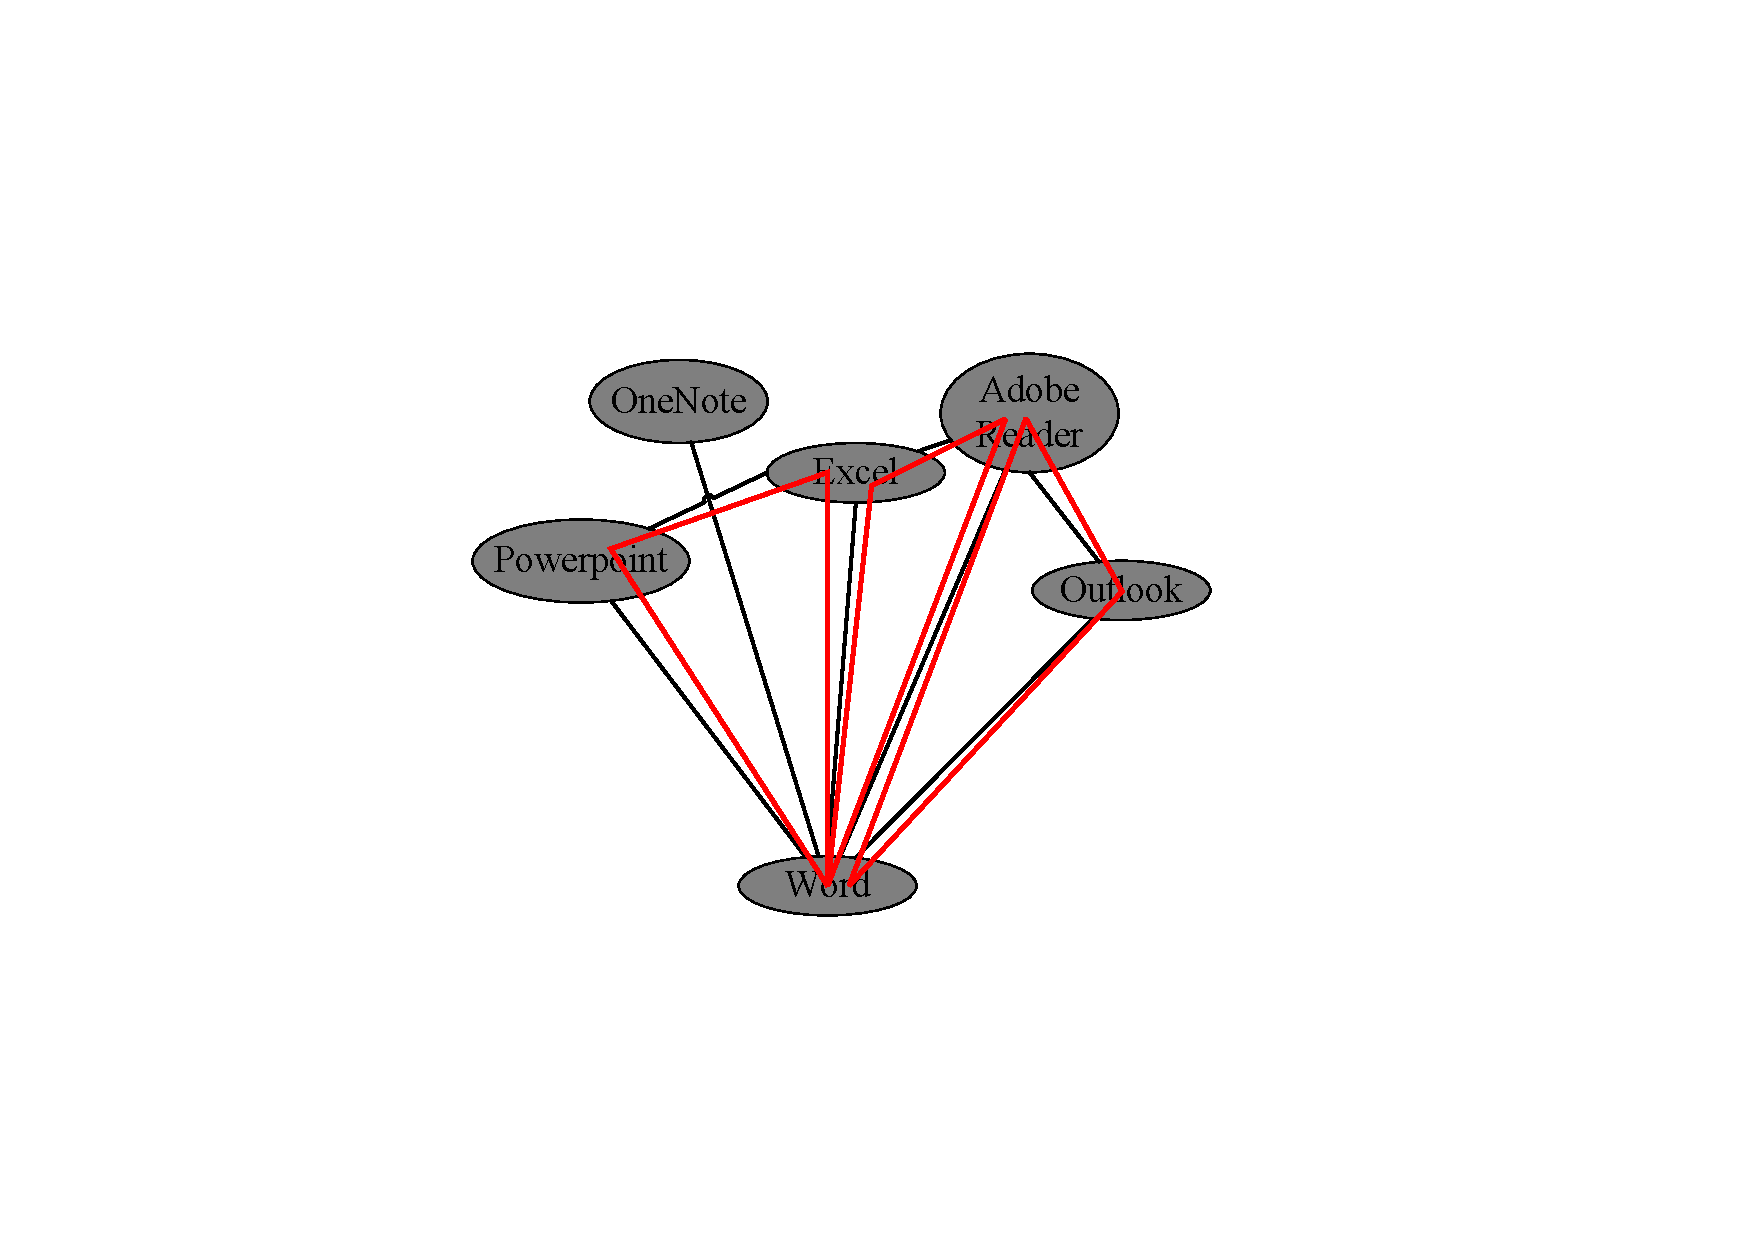
\includegraphics[angle=270, width=.45\linewidth]{img/chap3/LCC.pdf}}
% \hspace{0.1in}
\quad
\subfigure[Photoshop]{\label{fig:lcc:ps} 
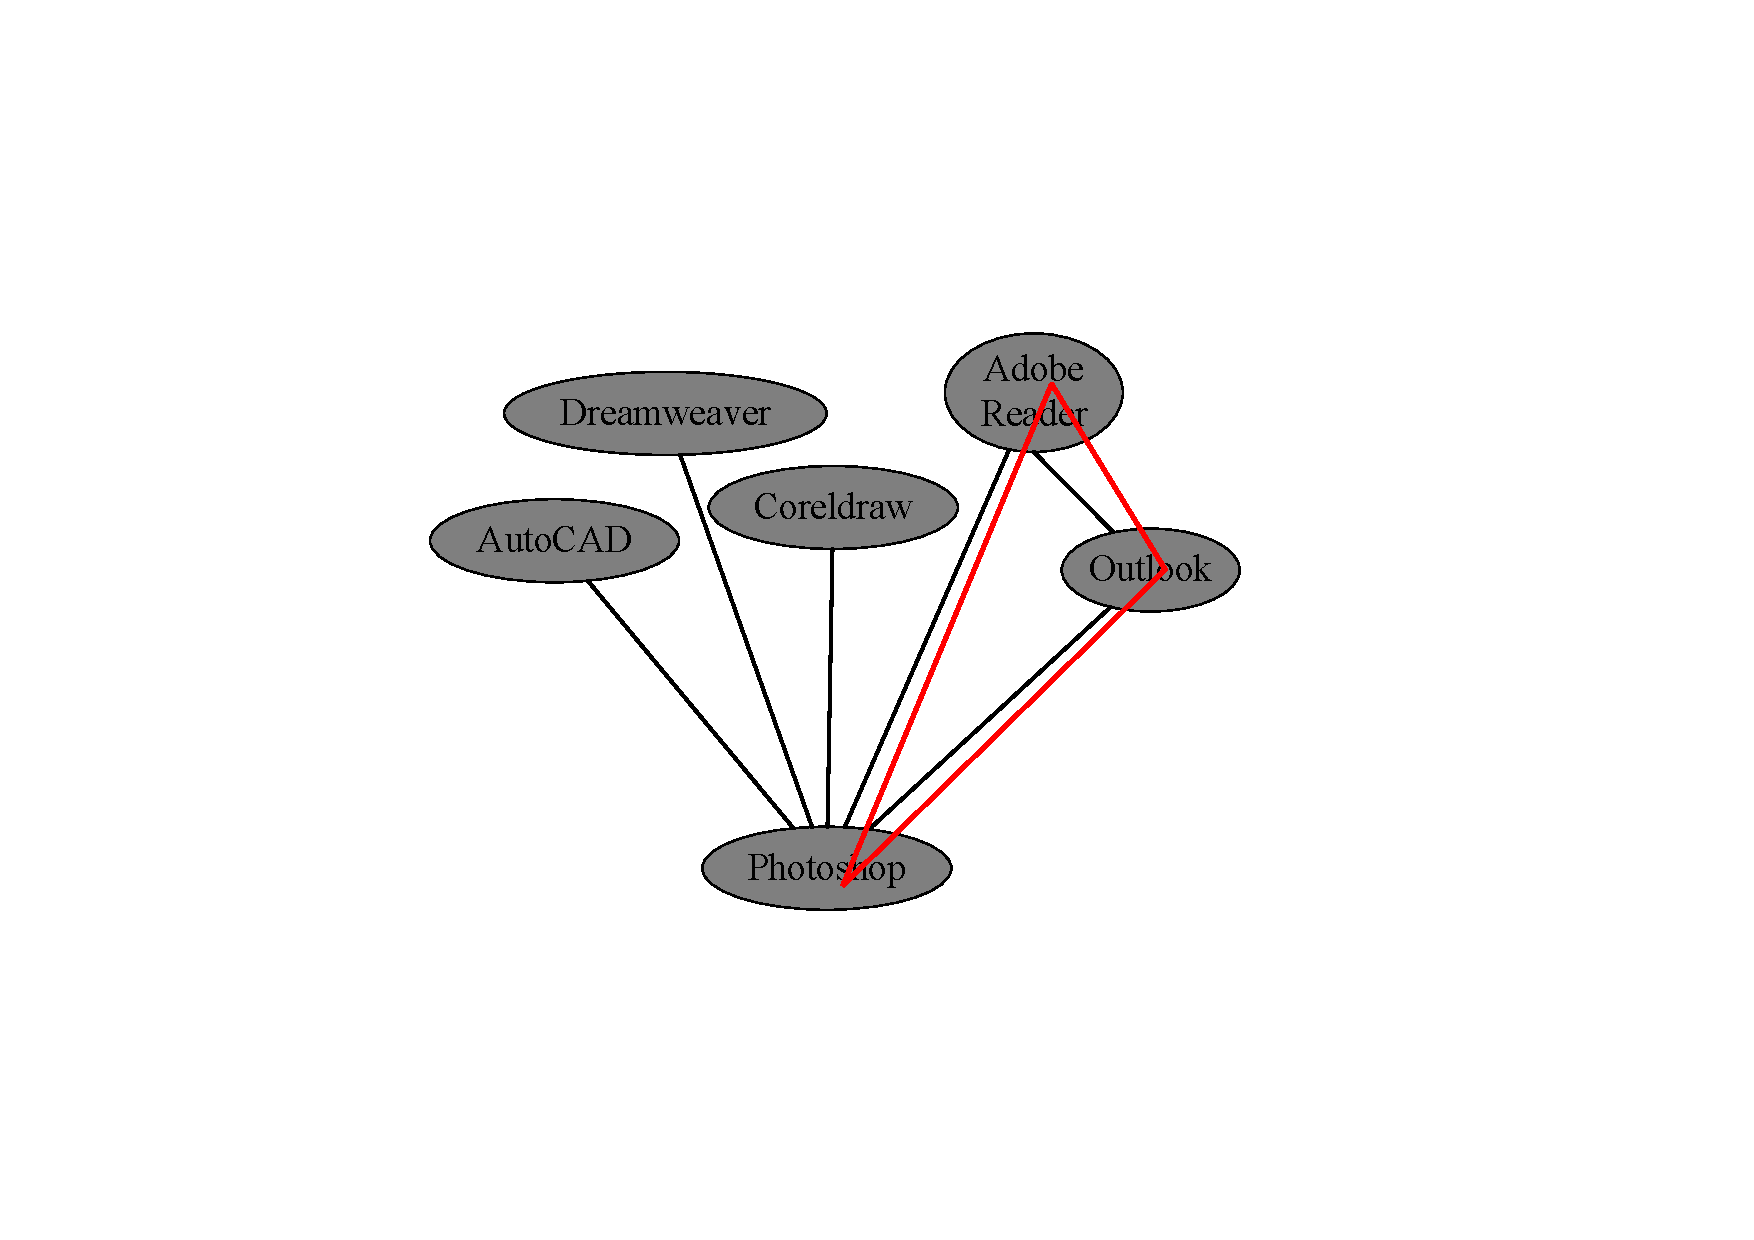
\includegraphics[angle=270, width=.45\linewidth]{img/chap3/LCC_low.pdf}}
\caption{``Word''和``Photoshop''局部聚类系数对比}
\label{fig:lcc}
\end{figure}

\subsubsection{度中心性}
度中心性(Degree Centrality)是在网络分析中刻画节点中心性(Centrality)的度量指标。一个节点与越多的节点发生直接联系,节点的节点度就越大,就意味着节点的度中心性越高,那么这个节点就处于中心地位,在网络中就越重要\cite{scott2012social}。
\begin{equation}
DC(v)=\frac {d_{v}} {n-1}
\end{equation}
其中,$n-1$为节点$v$可能连接的最大节点数,$n$为图中节点的数量。

\subsubsection{接近中心性}
接近中心性反应了节点在网络中与其他节点之间的接近程度,体现了节点对图的全局认识程度。具有较高接近中心性的节点能够比其他节点更快速的触及整个图。
\begin{equation}
CC(v)=\frac {n-1} {\sum_{u \neq v}^{n}g(u,v)}
\end{equation}
其中,$g(u,v)$是节点$u$和$v$之间的最短路径,$n$为图中节点的数量。

\subsubsection{中间中心性}
中间中心性体现了一个节点在图中的地位。中间中心性的概念由Linton于1977年提出,用来衡量一个人在社交网络中控制他人信息交流的能力\cite{freeman1977set}。如果一个节点处在许多节点互联的路径上,可以认为此节点处于重要地位,因为该节点具有控制其他节点交互的能力,其他节点之间的交互需要通过该节点才可以进行。出现在很多其他节点之间最短路径上的节点将比其他的节点拥有更大的中间中心性。节点$v$的中间中心性可以根据公式\ref{eq:bc}计算,$\delta_{st}$是从节点$s$到节点$t$的最短路径总数,$\delta_{st}(v)$为从节点$s$到节点$t$的最短路径中经过节点$v$的路径个数,$n$为图中节点的总数。
\begin{equation}
\label{eq:bc}
BC(v)=\frac {1} {(n-1)(n-2)}\sum_{s \neq v \neq t \in V} \frac {\delta_{st} (v)} {\delta_{st}}
\end{equation}

\subsection{基于图属性的文件采样}
根据文件社交网络的关系以及每个文件所处位置可以看出,每个文件的重要性是不同的,重要性较高文件的邻居通过这些文件产生关联关系。因此,根据图的特征属性从大量的未标记文件集中选取具有代表性的重要的文件进行标记对于提高恶意软件检测的准确率和性能是十分重要的。本章选择度中心性(DC)、局部聚集系数(LCC)和接近中心性(CC)作为衡量文件重要性的因子,定义文件的重要性为:
\begin{equation}
importance(v_{i}) = \frac {DC(v_{i}) * LCC(v_{i})} {CC(v_{i})}
\end{equation}
该值越大,文件的重要性越大。根据重要性对未标记文件进行降序排序,选取前$k$个文件作为采样样本交由安全专家进行标记并加入已标记样本中来训练分类器。

\section{主动学习}
在传统的数据挖掘算法中,学习算法以给定的已标记样本数据集作为训练集进行训练学习。然而在很多现实的应用中,往往面临的情况是大量的未标记样本和极少量的已标记样本,而且未标记样本比已标记样本更加容易获取。对样本进行标记工作的成本是高昂的和困难的,需要花费大量的人力、物力和财力。Zhu等人研究表明\cite{zhu2005semi},对于训练样本的准确标记不仅需要数据的领域知识和领域专家,而且样本标记工作所需的时间是获取数据所花费时间的10倍以上。根据PAC学习理论,已标记样本的数量越多,算法的泛化误差越小,因此稀少的已标记样本使得现有的监督学习算法的应用能力大大降低。主动学习(Active Learning)算法被提出以有效地解决这类问题。主动学习算法模拟了人类的学习过程,通过选择重要的未标记样本进行标记并加入训练集,迭代学习来提高分类器的学习能力。
\subsection{相关概念}
主动学习是最早由Angluin等人在1988年提出\cite{angluin1988queries},其主要的思想根据数据分布情况,主动选择对分类器模型有重要意义的样本,交由领域专家进行人工标注并把这些样本加入到已标注的训练集中,通过反复的迭代学习训练,使得分类器拥有更好的泛化能力和分类准确率。

主动学习算法一般包括以下两个部分:
\begin{asparaenum}
\item 学习引擎(Learning Engine)。学习引擎在已标记样本集上训练一个分类器,当分类器的准确率或某一度量标准满足条件时结束训练并输出结果。
\item 采样引擎(Sampling Engine)。采样引擎根据学习引擎分类器的分类结果和一种样本选取策略在未标记样本集中选取样本,将样本交由领域专家进行人工标记,并在标记完成后将样本加入到已标记样本集中。
\end{asparaenum}

学习引擎和选择引擎进行循环交替,经过多次循环之后学习引擎中分类器的性能逐渐提高,并在分类器达到一定的性能条件后终止。算法\ref{alg:activelearning}以伪代码的形式描述了主动学习算法的流程。

\begin{algorithm}[!ht]
\caption{主动学习算法伪代码描述}
\label{alg:activelearning}
\begin{algorithmic}[1]
\Input 已标记样本集$L$,未标记样本集$U$,学习引擎$LE$,采样引擎$SE$
\Output 学习引擎$LE$
\Repeat
\State $LE.train(L)$\Comment{在已标记样本集上训练分类模型}
\State $T=LE.predict(U)$\Comment{}
\State $Q=SE.query(U, T)$
\State $Label(Q)$
\State $L=L+Q$
\State $U=U-Q$
\Until {性能条件$Condition$满足}
\end{algorithmic}
\end{algorithm}

采样引擎是整个主动学习过程的核心,根据采样引擎的不同,主动学习算法可分为三类:
\begin{asparaenum}
\item \textbf{成员查询综合(Membership Query Synthesis)}。成员查询综合是主动学习最早被提出的采样方案\cite{angluin1988queries}。算法通过学习器来生成一个样本,并交由专家进行标注。该方法的缺点是忽略了样本集的实际分布情况,有可能生成了人类专家无法标注的样本。
\item \textbf{基于流的主动学习(Stream-based)}。如图\ref{fig:al:stream}所示,基于流的主动学习从真实的样本空间中抽取样本,由选择算法决定是否需要将其交给专家进行标注,若不需要标注则舍弃。这种采样策略通常需要设定一个评价标准来对样本进行评估(例如一个固定的阈值),缺乏对不同应用场景的普适性。同时,算法过程中每次仅选取一个样本与阀值进行比较,忽略了与其他未标记样本的对比。
\item \textbf{基于池的主动学习(Pool-based)}。基于池的主动学习算法将未标记样本集看作一个``池'',每次从池中抽取最有价值的样本进行人工标注。基于池的主动学习解决了上述两种方法的缺点和不足,因此是当前研究最多、应用最广泛的样本抽取方法。图\ref{fig:al:pool}为基于池的主动学习算法过程。
\end{asparaenum}

\begin{figure}[!ht]
\centering
\subfigure[基于流的主动学习]{\label{fig:al:stream} 
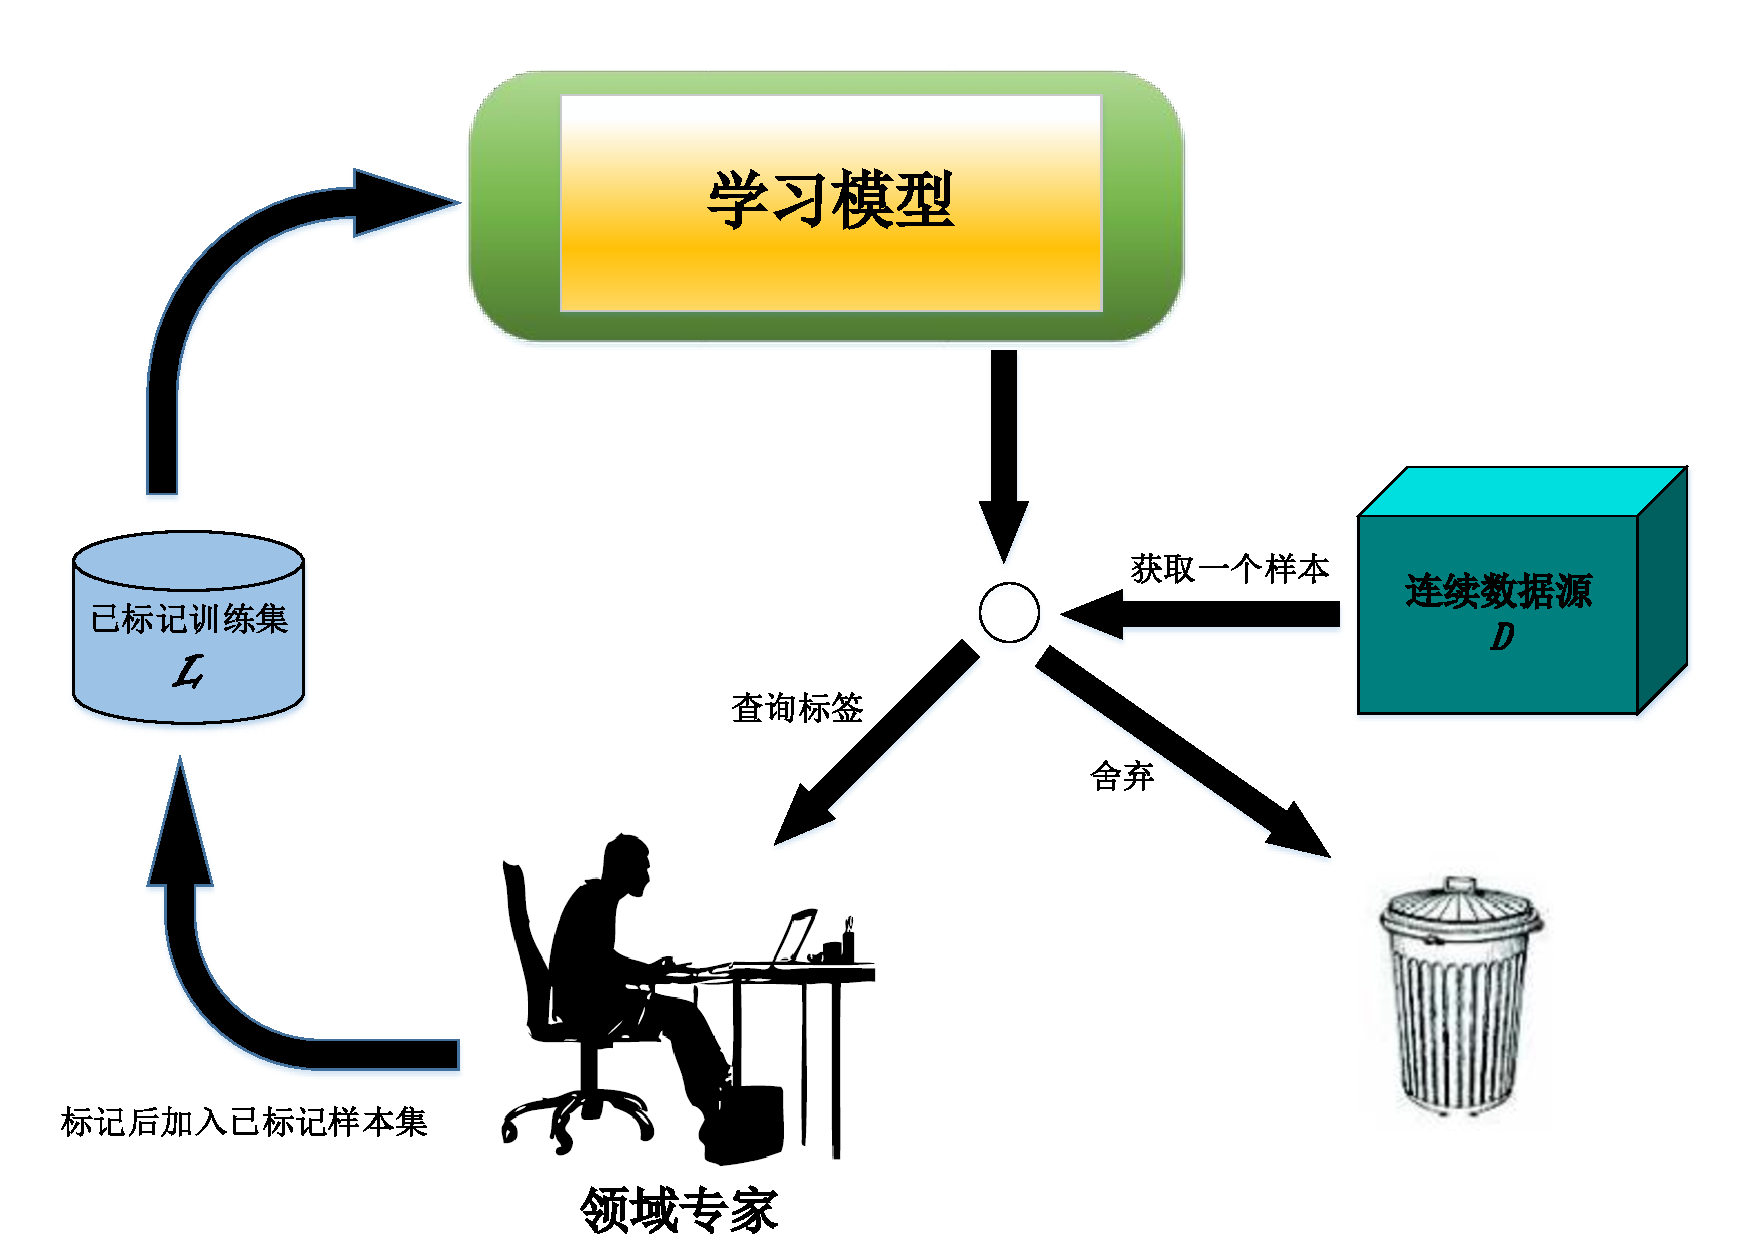
\includegraphics[width=.5\linewidth]{img/chap3/Stream_AL.pdf}}
\quad
\subfigure[基于池的主动学习]{\label{fig:al:pool}
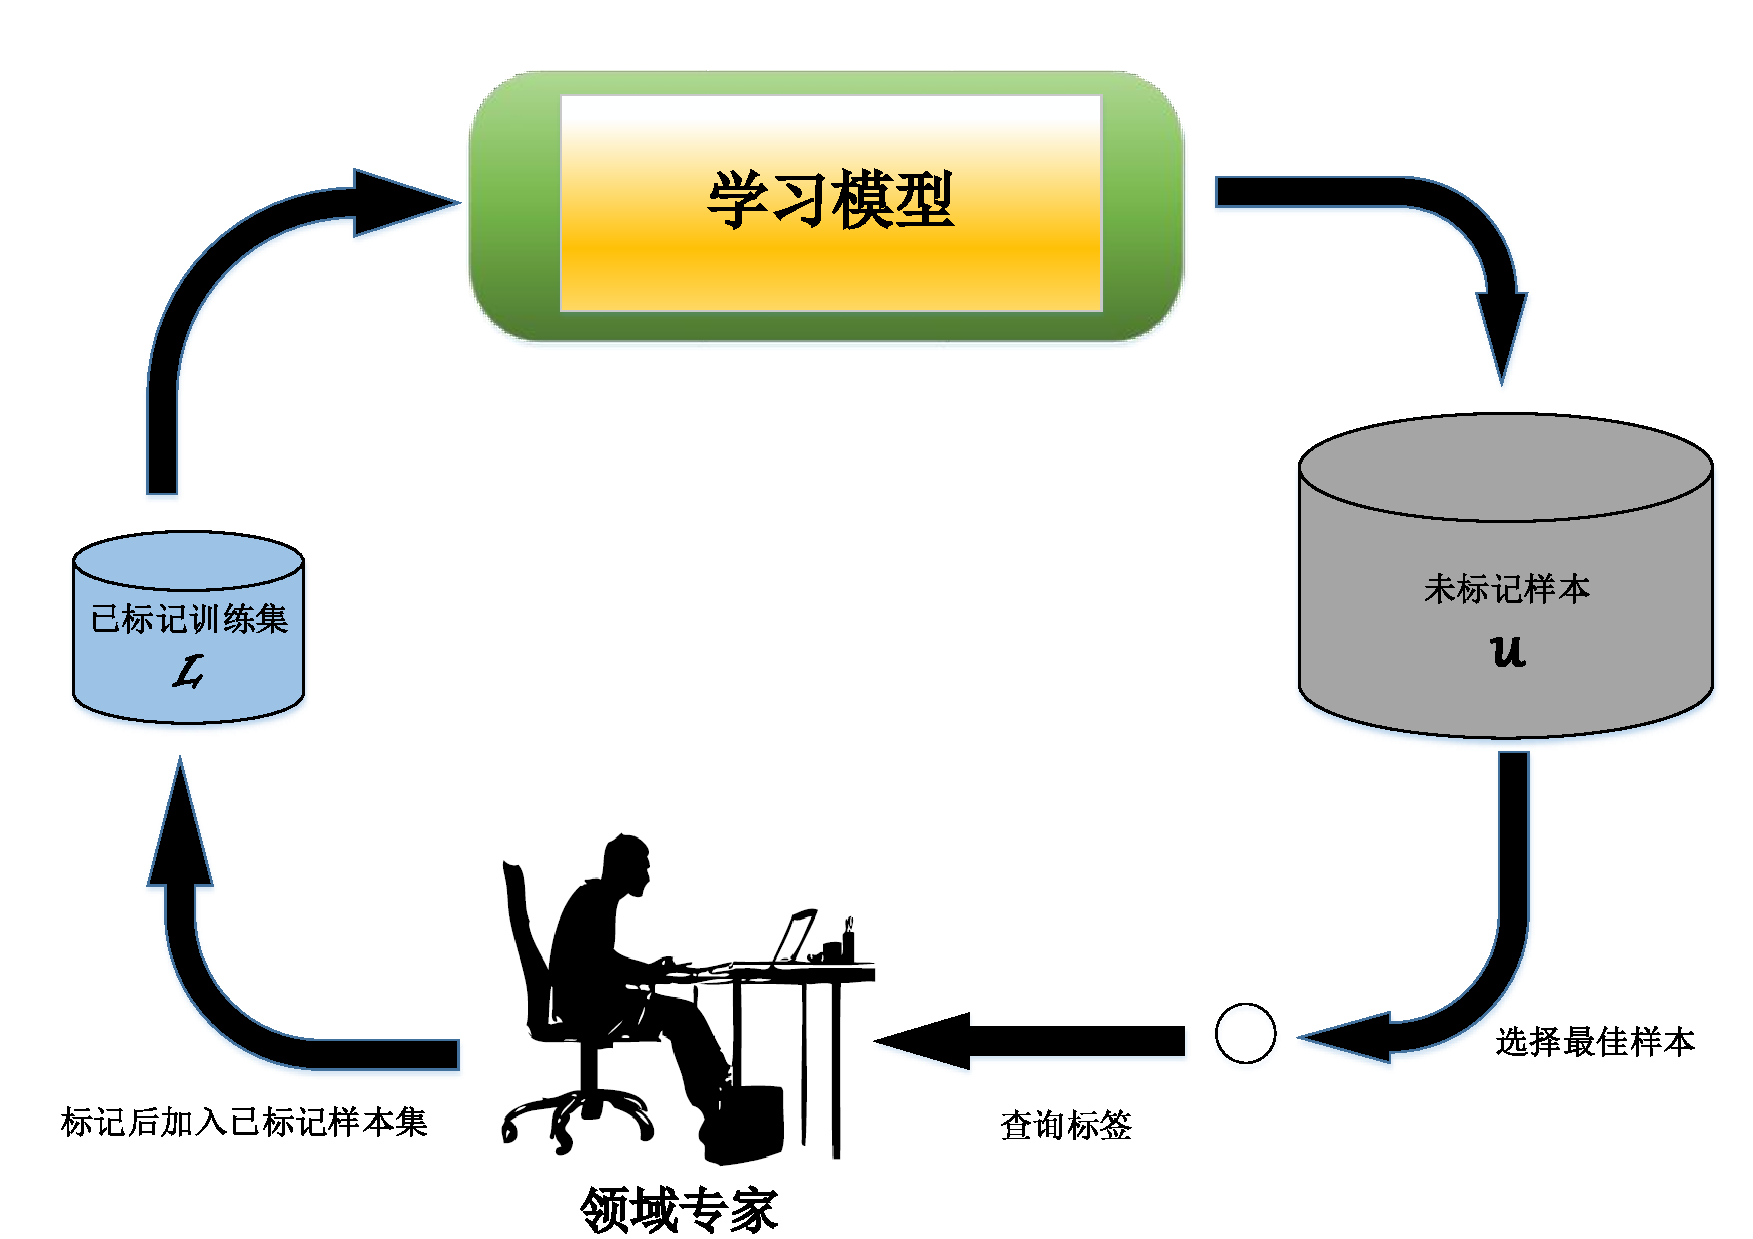
\includegraphics[width=.5\linewidth]{img/chap3/Pool_AL.pdf}}
\caption{主动学习示意图}
\label{fig:al}
\end{figure}

\subsection{主动学习算法采样策略}
近年来,众多的学者和工作聚焦于主动学习算法的研究,尤其是对样本选择算法的研究,希望能发掘出最有意义最具代表性的样本加入训练样本集。在上一节中,我们介绍了主动学习算法中采样方法的三种类型,其中基于池的主动学习算法是目前研究和应用最广泛的样本选择方法。因此,本章主要按照基于池的主动学习算法展开,根据样本选择标准的不同,主要介绍基于不确定性缩减、基于版本空间缩减和基于期望误差缩减三种样本选择策略。
\begin{asparaenum}
\item \textbf{基于不确定性缩减}。基于不确定性缩减的样本选择是目前研究较多的一种基于池的样本选择方法。这种选择方法选择当前分类器最无法确定标签的样本并交由专家进行标记。这种方法对于概率学习模型来说最简单适用。例如,对于二分类问题的概率模型来说,基于不确定性缩减的采样策略将选取那些后验概率接近0.5的样本\cite{lewis1994heterogeneous}。对于分类器来说,最无法确定标签的样本也是分类器最有可能产生分类错误的样本,选择这类样本进行人工标记,不仅能够有效减少人类专家的标注工作,也能较好地提高分类器的准确度和泛化能力。根据分类器模型的不同,衡量样本不确定性的方法和角度也有不同,因此采样策略也会不同,目前常用的方法包括最小边界、最低确定度、最小边缘、最大信息熵等。信息熵(Entropy)\cite{shannon1948math}是编码分布所需信息量的信息论度量,因此通常被认为是机器学习中不确定性或不纯度的度量:
\begin{equation}
x_{H}^{*}=\underset{x}{\arg\max}-\sum_{i}P_{\theta }(y_{i}|x)\log P_{\theta}(y_{i}|x)
\end{equation}
其中,$y$为所有的标签集合。基于信息熵的采样策略受到了广泛的研究和应用\cite{culotta2005reducing,hoi2006large},适用于各种复杂模型和多类别问题,在自然语言处理、文本分类等领域均有较好的性能。基于不确定缩减的采样策略可以应用于多种分类器模型,如逻辑回归(Logistic Regression)、隐马尔科夫模型(Hidden Markov Model)以及支持向量机(Support Vector Machine)等,在多数问题上都能获得较好的性能。
\item \textbf{基于版本空间缩减}。版本空间是概念学习中与已知训练集一致的所有假设(Hypothesis)的子集集合,因此学习器所需要训练的目标假设肯定也包含其中。基于版本空间缩减的主动学习样本选择方法的目的就是选择那些能够最大程度地缩减版本空间的样本进行标记。委员会投票选择算法(Query By Committee, QBC)是一种典型的版本空间缩减的样本选择方法。首先,从当前的版本空间中随机地选择$C$个不同的假设构成一个委员会$Committee=\{\theta^{(1)},...,\theta^{(C)}\}$,委员会中的每个假设对所有未标记样本进行分类投票,选择各个假设分类结果差异最大的样本交由专家进行标记。换句话说,在当前的训练集上构建多个分类器模型,运用这些模型来预测未标记样本,并选择分类结果不一致性的样本进行标记。委员会投票选择算法的核心是如何衡量成员对样本的的不一致性程度。作为最早提出的QBC算法\cite{seung1992query},Seung等人采用投票熵作为评价委员会成员分类差异度的标准:
\begin{equation}
x_{VE}^{*}=\underset{x}{\arg\max}-\sum_{i}\frac {V(y_{i})} {C}\log \frac {V(y_{i})} {C}
\end{equation}
其中,$y_{i}$为所有可能的类别,$V(y_{i})$是投票为$y_{i}$的委员会分类器个数,$C$是委员会的分类器个数。McCallum等人将样本分布密度与QBC相结合的EM-QBC算法,引入KL分歧度(Kullback-Leibler Divergence)作为衡量两个概率分布差异程度的标准,计算方法如下:
\begin{equation}
KL(p_{1}(x),p_{2}(x))=-\sum_{i\in L}p_{1}(x_{i})\log\left (\frac {p_{1}(x_{i})} {p_{2}(x_{i})}  \right )
\end{equation}
该算法的主要思想是委员会成员中不一致性程度最大的样本分布区间包含拥有最大信息量的样本。算法将这一区间内的样本交由专家进行标记。另外,委员会的建立策略也是研究的一个重点,Abe采用集成学习中Boosting和Bagging方法提出了Boosting-QBC和Bagging-QBC的委员会建立策略\cite{naoki1998query}。
\item \textbf{基于期望误差缩减}。主动学习的目的是通过选择最优样本进行标记并加入训练来降低分类器的误差和提高分类器的分类准确率。基于期望误差缩减的样本选择方法就是通过减少分类器的误差来直接提高算法的泛化能力。该方法选择使得分类器未来泛化误差最大程度缩减的样本进行标记。具体步骤为:采样算法将每一个未标记的样本都作为候选样本,将其标记后加入已标记样本训练集并训练分类器;对比分类器训练前后的误差变化,选择能够最大程度缩减分类器泛化误差的样本进行标记并加入已标记样本集。Cohn等人\cite{cohn1996active}提出了基于统计学的主动学习算法,采用了模型方差最小化的缩减策略,并在人工神经网络、高斯混合模型和回归模型中加以应用。基于期望误差缩减的方法,主要搜索使期望误差缩减最大化的未标注样例,来减少标注样例的次数并且有效提高分类器的性能,但是这种方法的计算量较大,尤其是数据集合较大的情况下。
\end{asparaenum}

大多数的主动学习算法致力于每次选择一个最优样本进行标记,在标记后重新训练模型并循环这一过程(采样$\rightarrow$标记$\rightarrow$训练)直至达到迭代次数或满足性能优化要求。然而,很多模型的训练优化是复杂而且耗时的,从而反复训练模型的代价是高昂的,而且如此反复的训练模型在实际的运用中也是不现实的,因此提出了批量模式的主动学习算法。批量模式的主动学习不仅能够减少采样冗余,而且还可以增加样本的多样性。Hoi等人通过最大化查询批量样本的费舍尔信息来解释冗余问题\cite{hoi2006large,hoi2006batch}。

主动学习作为解决数据稀缺问题的有效范例,通过领域专家反馈信息优化了分类器的学习效果,降低了监督学习获取数据标签信息的成本,近年来已经受到广泛关注和深入研究\cite{nguyen2004active,muslea2006active}。特别是随着在各种应用领域内图和网络数据的丰富,基于图的主动学习已经受到很多研究的关注\cite{cesa2010active,cesa2010activetreesandgraph,zhao2008scalable}。

\subsection{最大批量网络增益的采样算法}
最大批量网络增益采样是批量模式主动学习的优化采样策略,将代表性和多样性与传统的不确定性标准相结合。代表性和多样性考虑了训练集中的实例之间的相互依存关系,是不确定性标准的两个补充标准。在选择待标记样本时,样本需要具有代表性以能够提高分类器模型的性能,同时也可以具有更大的多样性以降低标记操作的冗余。最大批量网络增益采样结合代表性和多样性两个特点,并通过最大化网络增益来选择批量样本集。

对于未标记样本集$U$中的每个样本$x_{i}$,查询样本的标签信息的个体信息增益通过信息熵计算:
\begin{equation}
H(x_{i})=-\sum_{y}P(y|x_{i})\log P(y|x_{i})
\end{equation}
其中,$P(y|x_{i})$是标签传播算法计算得到的样本$x_{i}$标签分布概率。

根据标签传播算法,查询批次的网络增益通过传播查询本批次中每个样本的个体信息增益至图中其他的未标记样本来计算,因此定义批量网络增益$NG(B)$为:
\begin{equation}
\label{eq:ng}
NG(B)=\sum_{j \in U-B,i \in B}w_{ji}H(i)-\mu \sum_{i,k \in B,i \neq k}w_{ki}H(i)
\end{equation}
其中,第一部分代表了从剩余未标记样本中查询批量样本的信息增益,而第二部分表示批次内样本之间的冗余,$w_{ji}$是节点$j$和$i$之间边的权重,$\mu$为惩罚因子。批量网络增益结合了不确定性(节点信息熵$H(\cdot)$)、代表性(公式\ref{eq:ng}中第一部分)和多样性(公式\ref{eq:ng}中第二部分)。

在主动学习迭代过程的每一步,选择具有最大网络增益$NG(B)$的样本批次来交由领域专家进行标记。定义$W=[w_{ij}]$为图的邻接矩阵,可以将公式\ref{eq:ng}中第一部分的最大化问题转化为在给定$B$大小的情况下最大化分割图中$B$和$U-B$的问题。通过贪心算法可以求解该问题,伪代码描述如算法\ref{alg:ngal}所述。
\begin{algorithm}
\caption{最大批量网络增益采样}
\label{alg:ngal}
\begin{algorithmic}
\Input 未标记样本集$U$, 批量大小$N$
\State $B=\emptyset $  \Comment{初始化$B$为空集}
\Repeat
\State $k={\arg\max}_{i \in U}{NG(B\cup {i})}$
\State $B\leftarrow B\cup {k}$, $U\leftarrow U-{k}$
\Until {$\left | B \right |=N$}
\end{algorithmic}
\end{algorithm}

\section{基于主动学习的标签传播算法}
上一节我们提出了一个基于批量模式的最大网络增益主动学习采样算法,结合标签传播算法的特点选取能够最大化提升标签传播算法性能的节点进行标记。整体算法描述如算法\ref{alg:allp}所示。
\begin{algorithm}
\caption{Label Propagation With Active Learning}
\label{alg:allp}
\begin{algorithmic}
\Input 未标记数据$D_{U}=(x_{l+1},y_{l+1})...(x_{l+u},y_{l+u})$, 标记数据$D_{L}=(x_{1},y_{1})...(x_{l},y_{l})$及类别集$C$
\Output 未标记数据的类别
\Repeat
\State $initial(D_{U}, D_{L})$ \Comment{初始化相似度矩阵$W$和标签传递矩阵$T$}
\For{$i=0; i<l+u; i++$} \Comment{初始化标签矩阵$Y$}
\For{$j=0; j<\left | C \right | ; j++$}
\State $Y_{ij} = p(y_{i},C_{j})$
\EndFor
\EndFor
\Repeat
\State $Y\leftarrow \overline{T}Y$ \Comment{传播标签信息}
\State $clamp(D_{L})$ \Comment{限定已标记数据}
\Until {$Y$ converges}
\State $B=\emptyset$  \Comment{初始化$B$为空集}
\Repeat
\State $k={\arg\max}_{i \in U}{NG(B\cup {i})}$
\State $B\leftarrow B\cup {k}$, $U\leftarrow U-{k}$
\Until {$\left | B \right |=N$}
\Until {the stopping criterion S is satisfied}  \Comment{直至满足迭代停止条件}
\State $assignLabel(D_{U})$
\end{algorithmic}
\end{algorithm}

\section{基于文件社交网络的恶意软件检测方法}
在分析了文件社交网络特点和特征属性的基础上,运用上一节提出的基于主动学习的标签传播算法可以分析文件之间标签信息传播的过程并进行恶意软件的检测。算法\ref{alg:findmal}描述了整个算法的流程。

\begin{algorithm}
\caption{基于文件社交网络的恶意软件检测方法}
\label{alg:findmal}
\begin{algorithmic}
\Input 原始文件列表数据$FileList$
\Output 文件样本的标签
\For{each $f_{i}$ in $FileList$}\Comment{计算每个文件与已知关联文件之间的相似度}
\State $similaityASS(f_{i})$
\EndFor
\For{each $f_{i}$ in $FileList$}\Comment{计算未标记文件样本之间的相似度}
\For{each $f_{j}$ in $FileList$}
\If{$f_{i}$ is unlabled and $f_{j}$ is unlabled}
\State $similaityUnLabel(f_{i},f_{j})$
\EndIf
\EndFor
\EndFor
\State $createGraph(V,E,W,k)$\Comment{构造$k$近邻图}
\State $samplingByGraphFeature(G)$\Comment{根据图属性选择重要文件样本进行标记}
\State 运用基于主动学习的标签传播算法训练
\State 根据标签矩阵标记未标记文件样本的标签
\end{algorithmic}
\end{algorithm}

\section{实验验证}
在本章中,我们提出了一种基于文件社交网络的恶意软件检测方法,由于部分方法和技术在上一章中已经进行了实验验证,故本章不再赘述。本节重点通过两组实验分别来验证基于图属性的文件采样方法和主动学习算法的可行性和有效性。

本章实验所用平台与上一章相同,在此不再赘述。在上一章分析实验结果时我们可以发现,由于数据的不均衡性,良性文件的数量远远大于恶意软件的数量,因此在准确率$ACC$的计算上良性文件的数量占据了主要成分,考虑以下两种极端情况:第一种情况,所有的文件(包括恶意和良性)都被判为良性文件,在这种情况下,算法的准确率$ACC$就可高达92.75\%,而$TPR$则为0;然而第二种情况,所有的文件都被判为恶意软件,此情况下算法的准确率$ACC$则为7.25\%,而$TPR$则为100\%。在本章中,综合考量各类别样本的分布情况,选择以下性能评价指标以体现算法的性能:
\begin{itemize}
\item \textbf{Recall}: $\frac {TP} {TP+FN}$: 正确标记为恶意的样本占恶意软件总量的比率。
\item \textbf{Precision}: $\frac {TP} {TP+FP}$: 标记为恶意软件的样本中确为恶意样本的比率。
\item \textbf{Accuracy(ACC)}: $\frac {TP+TN} {TP+TN+FP+FN}$
\item \textbf{F1-Score}: $\frac {2\cdot precision \cdot recall} {precision + recall} = \frac {2TP} {2TP+FP+FN}$.
\end{itemize}

\subsection{基于图属性的采样策略分析}
本章提出了三个基于图的特征属性,根据这些属性衡量文件的重要性,并选择具有高代表性的文件交由安全专家进行标记。本节将通过实验来验证这三个属性以及采样算法对算法提升的作用。实验中,分别比较基于局部聚集系数(Local Clustering Coefficient)、度中心性(Degree Centrality)、接近中心性(Closeness Centrality)以及综合三个属性的$important$值采样和随机抽取方法对算法的性能改善能力。从表\ref{tb_EvaGF}可以看出,综合三个图属性的$important$对分类器性能的提升有最好的作用。为了中和方差,随机抽取方法运行十次,取平均值作为最终结果。

\begin{table}[!ht]
\renewcommand{\arraystretch}{1.5}
\caption{基于图属性的采样策略分析}
\label{tb_EvaGF}
\centering
\begin{tabular}{ccccc}

\toprule
Feature & Recall(\%) & Precision(\%) & ACC(\%) & \textbf{F1-Score(\%)}\\
\midrule
Random & 50.3 & 67.0 & 94.2 & 57.4 \\
DC & 50.1 & 67.5 & 94.1 & 57.5 \\
CC & 49.8 & 68.4 & 94.4 & 57.7 \\
LCC & 50.8 & 66.3 & 94.2 & 57.5 \\
Combination & 50.7 & 68.0 & 94.2 & \textbf{58.1} \\
\bottomrule
\end{tabular}
\end{table}

\subsection{主动学习对预测的影响}
在本实验中,将系统性地分析和评估主动学习算法对分类器的影响。为了验证最大批量网络增益采样策略的有效性,选取随机抽样策略作为对比策略。最大批量网络增益算法的批量大小设置为20,即每次从未标记数据集中选择20个最代表性的样本进行标记。同理在随机抽样策略中,每次也从未标记数据集中抽取20个样本进行标记。

\begin{figure*}[!ht]
\centering
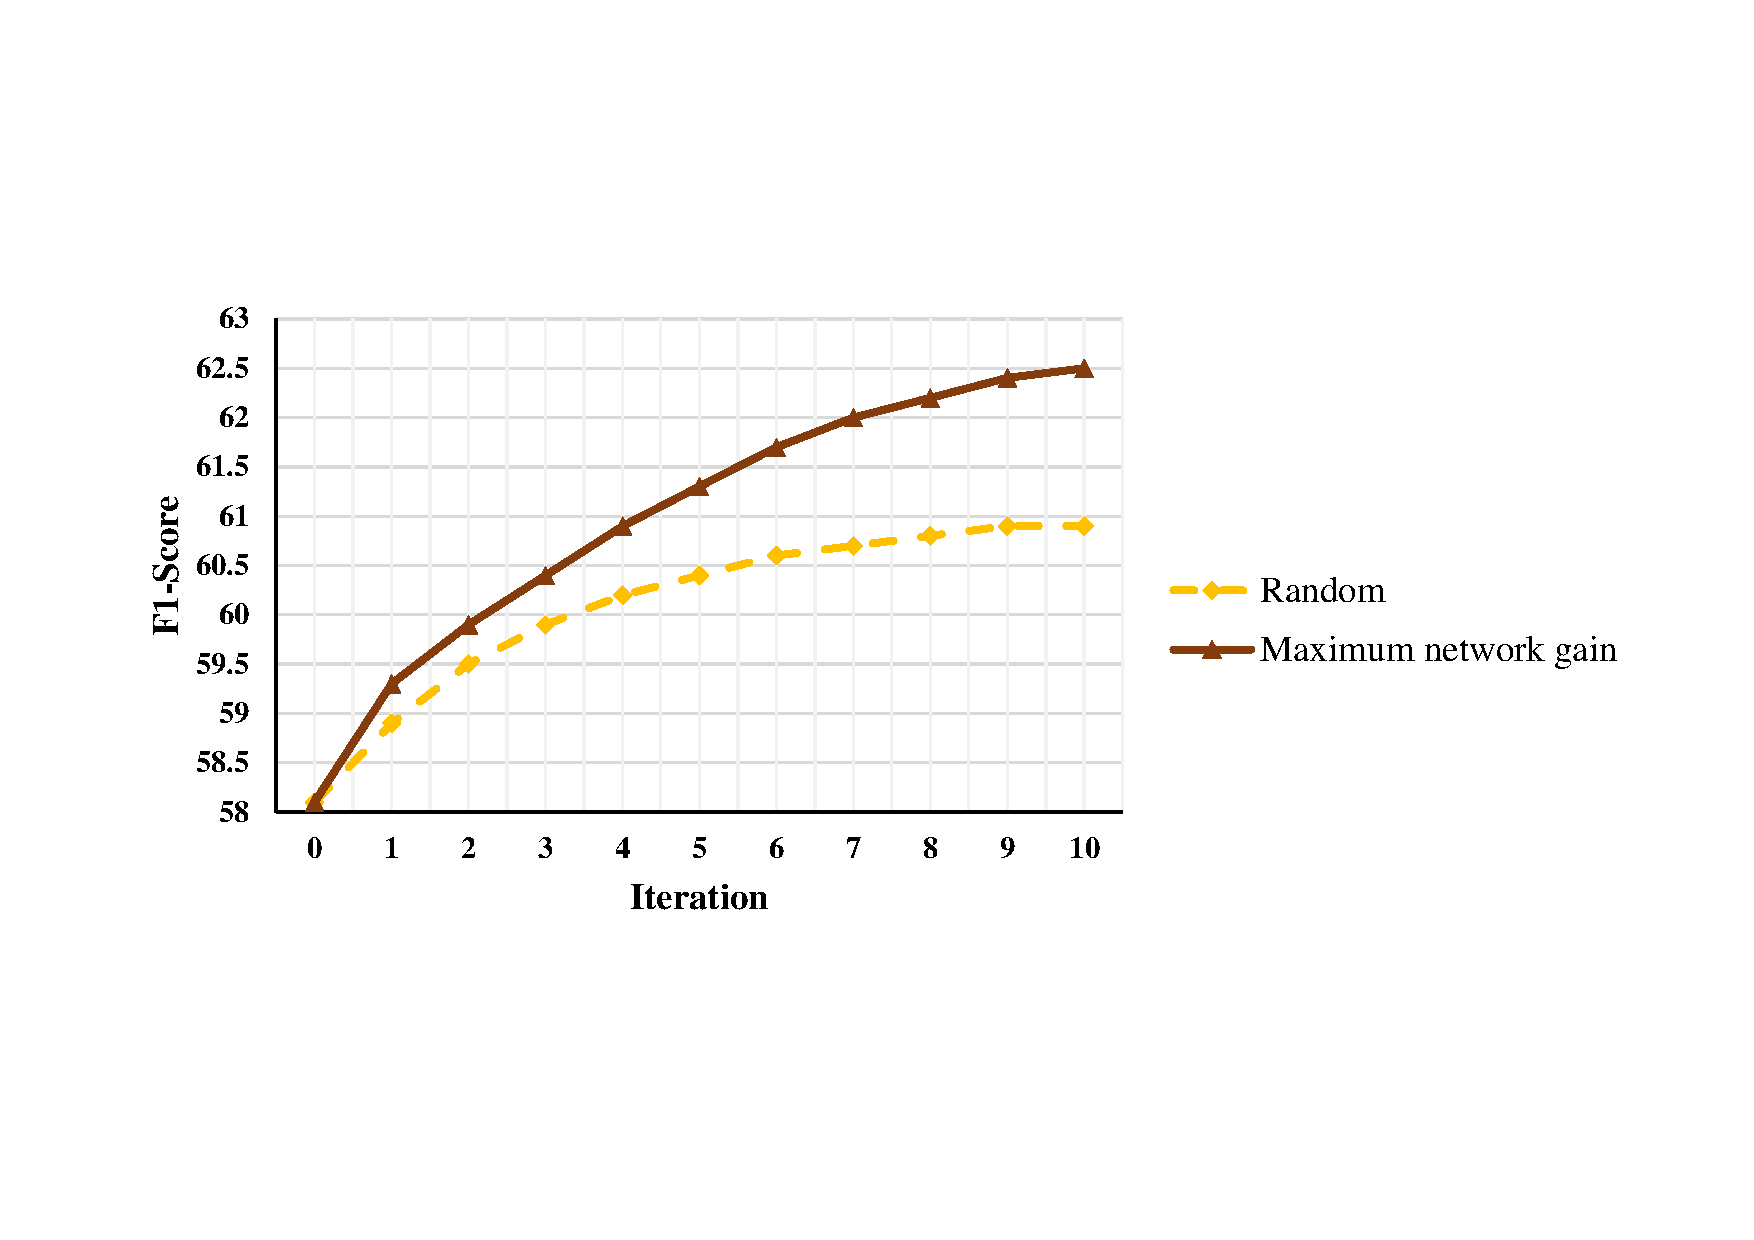
\includegraphics[width=5in]{img/chap3/AL_Comparison.pdf}
\caption{主动学习算法对预测的影响}
\label{fig_ResALComparison}
\end{figure*}

从图\ref{fig_ResALComparison}中可以看出,结合了最大批量网络增益采样策略主动学习算法的标签传播算法能够比随机采样有更好的表现。从第三次迭代开始,最大批量网络增益的主动学习算法与随机采样策略之间的差距逐渐变大,这样的趋势也表明本章提出的恶意软件检测系统的性能比其他的方法要好。

\section{本章小结}